\subsection{Data Visualization}\label{subsec:data-visualization}

Data visualizations are a vital part of data analysis, and data can be visualized in several ways, all depending on the
type of data in question and the parameters of interest.
Since one of this project's core focuses is business intelligence, it is of vital importance to understand different
data visualization strategies and select the one that best covers the client's needs.
This section will explore the visualization requirements as set by the client, and the raw data given to the group by
the client, since it forms the basis for any visualization strategy.
The client provided specific initial requirements, which the study group further interpreted and expanded upon to
develop additional requirements based on the client's underlying needs and objectives.
Furthermore, this section will investigate the different types of data visualizations available, while focusing on the
types of visualizations that meet the client's criteria.

\subsubsection{The Raw Data}\label{subsubsec:the-client's-raw-data}
The raw input data merely consists of order data from the client's~\acrshort{epos} system.
The~\acrshort{epos} system lacks data pre- and post-processing or categorization features, so all data collected by the
system is persisted directly ``as is'', i.e., orders are saved directly as individual entries in a database.
Orders, e.g., include attributes such as transaction time, a unique order ID, the product IDs of the products purchased,
and various other identifiers.
Due to the raw and uncategorized, unprocessed nature of the data, it will be necessary not only to visualize the data in
the software solution, but also process it first.

\subsubsection{Requirements}\label{subsubsec:requirements}
Specific requirements for the type of chart were not mentioned by the client during initial consultations, other than it
should be easy to understand even for student workers and other staff.
Given that none of the staff has knowledge about data science or analysis, it can be deducted that a type of chart will
have to be used that doesn't require specific skills in data interpretation.

Another important aspect is the type of information that the client wants to be able to understand from the
visualizations, namely, how sales change over time, and if there exists any specific pattern to the changes in sales.
Such patterns could, e.g., be that customers are more frequent on a specific day or at a specific time of day, or that
sales increase during holiday periods.

And in tandem with that lies the client's underlying objective to optimize their business.
The data visualization should serve the purpose of letting the client understand how to optimize their café's food
preparation and inventory sourcing.

\subsubsection{Static vs.\ Dynamic Visualizations}\label{subsubsec:static-vs-dynamic-visualizations}
Data visualizations can broadly be categorized into static and dynamic visualizations.
Static visualizations, as the name implies, don't have any interactive features that make it possible for the viewer to
edit or otherwise interactively modify the data and visualization in real time.
Such visualizations are optimal for printed or other static mediums.
Since static visualizations can only capture a specific moment in time~\cite{wpDataTablesDynamicVisualization}, they are
seemingly easier to decode, since the viewer only needs to understand a single perspective on the data.
Dynamic visualizations, on the other hand, offer more features, but require a dynamic environment.
They potentially can display multiple points in time and let the user interact with the data until a desired view is
achieved~\cite{wpDataTablesDynamicVisualization}.
One drawback of dynamic visualizations, though, is the additional requirements placed on the viewer, who is now partly
responsible for filtering and displaying the data.
But granted that the data has been sufficiently pre-processed by the software application, the client's requirement of
easy to understand visualization can still be met.
Additionally, since the client's data will eventually be visualized in an interactive web application, it could be
considered to use a dynamic visualization.

\subsubsection{Relevant Visualization Types}\label{subsubsec:relevant-visualization-types}
A handful of visualization types exist, and all of them serve different purposes.
Visualizations can further broadly be categorized into charts, plots and maps.
There are four traditional chart types: Bar and line chart, and scatter and box plot~\cite{atlassianChartTypes}.
Since we already established that we are interested in understanding relationships between data variables, we will now
focus on chart types that can help us exactly with that.

\pagebreak

% textidote: ignore begin
\begin{wrapfigure}{r}{0.4\textwidth}
    \centering
    \includegraphics[width=0.38\textwidth]{scatter-plot}
    \caption{A typical scatter plot~\cite{atlassianChartTypes}.}\label{fig:scatter-plot}
\end{wrapfigure}
% textidote: ignore end
Demonstrations of the relationship between two variables are a typical application of the \textit{scatter plot}
as seen in Figure~\ref{fig:scatter-plot}, which has two axes, one for each variable.
The dots on the plot itself are coordinates at which there is a correlation between the variables.
In the case of the café, such a plot could be used to analyze the sales vs.\ time of day or sales vs.\ day of the week
relationships.
E.g., where one axis, the y-axis, signifies sales, and the x-axis the time of day.
A high number of dots in a specific area of the plot, or \textit{clustering}, signifies a high correlation between the
variables at those points.
Such a plot could help the client analyze if there is any clustering at a specific time of day, or day of the week.

% textidote: ignore begin
\begin{wrapfigure}{r}{0.4\textwidth}
    \centering
    \includegraphics[width=0.38\textwidth]{line-chart}
    \caption{A line chart~\cite{atlassianChartTypes}.}\label{fig:line-chart}
\end{wrapfigure}
% textidote: ignore end
Another type of chart is the \textit{line chart} in Figure~\ref{fig:line-chart}, which, again, has two axes: One for
each variable.
Line charts are perfect for representing time series data, since they clearly visualize peaks and dips in the data.
If we, again, want to visualize the relationship between sales and time of day, sales could be plotted on the y-axis,
while the time of day would be on the x-axis.
A chart peak would then signify a peak in sales at a given point of time during a specific day.
Furthermore, such a chart could also be used for longer time intervals, such as a whole month, to analyze on which date
sales peaked or diminished.

% textidote: ignore begin
\begin{wrapfigure}{r}{0.4\textwidth}
    \centering
    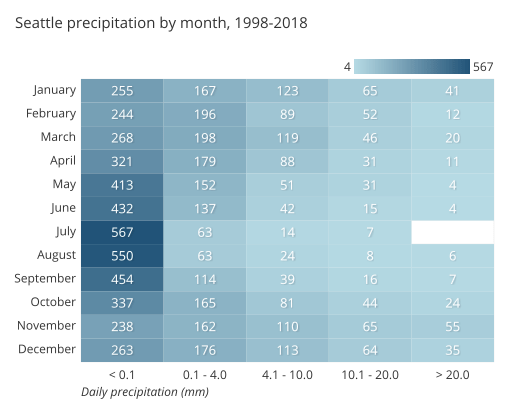
\includegraphics[width=0.38\textwidth]{heatmap}
    \caption{A heatmap~\cite{atlassianHeatmaps}.}\label{fig:heatmap}
\end{wrapfigure}
% textidote: ignore end
The final type of visualization that we will discuss here is the \textit{heatmap} as can be seen in
Figure~\ref{fig:heatmap}.
Heatmaps offer 2-dimensional representations of three or more variables and are therefore more flexible and can
potentially give more insight into the data at hand.
Figure~\ref{fig:heatmap} shows a typical heatmap, where the months of the year are mapped along the y-axis, while the
x-axis shows the daily precipitation.
The third variable, namely the amount or intensity of precipitation, is the color gradient of the blue cells.
A darker color is associated with higher amounts of precipitation, while a lighter color with fewer amounts.
In the context of the café problem, the y-axis could, e.g., display the day of the week, while the x-axis could display
the sales or revenue.
The color gradient would then signify the customer activity, with darker colors representing higher sales.
